\documentclass[11pt]{article}
\usepackage{asd-stile}

% ---- pacchetti specifici della relazione --------------------
\usepackage{graphicx}      % grafici della sperimentazione
\usepackage{booktabs}      % tabelle pulite
\usepackage{hyperref}
\hypersetup{colorlinks=true, linkcolor=asdblu, urlcolor=asdblu, citecolor=asdblu}

% Riserva spazio in fondo alla pagina: se non ne resta abbastanza si passa
% alla pagina nuova. Evita che un box di pseudocodice si spezzi a met\`a.
% (equivalente minimale di \Needspace: il pacchetto needspace non c'\`e
%  in questa installazione TeX Live)
\usepackage{fancyvrb}
\newtcolorbox{codice}{breakable,enhanced,colback=asdgrigiosoft,
  colframe=asdgrigio!45,boxrule=0.4pt,arc=2pt,
  left=8pt,right=8pt,top=6pt,bottom=6pt}

\makeatletter
\newcommand{\servespazio}[1]{%
  \begingroup\setlength{\dimen@}{#1}%
  \vskip\z@\@plus\dimen@ \penalty-100 \vskip\z@\@plus-\dimen@ \endgroup}
\makeatother

\begin{document}

% ============================================================
%  FRONTESPIZIO
% ============================================================
\begin{titlepage}
\centering
\vspace*{2cm}
{\sffamily\color{asdblu}\Large Algoritmi e Strutture Dati\par}
{\sffamily\color{asdblu}\large Elaborato a.a.\ 2025--26\par}
\vspace{2.6cm}
\rule{\linewidth}{1pt}\par\vspace{8pt}
{\sffamily\color{asdblu}\Huge\bfseries Problema dello Zaino 0/1\par}
\vspace{10pt}
{\sffamily\large Risoluzione con programmazione dinamica\\[2pt]
e confronto con un solver ILP\par}
\vspace{8pt}\rule{\linewidth}{1pt}
\vspace{2.6cm}

{\large Marco Cesari\par}
\vfill
{\large \today\par}
\end{titlepage}

% ============================================================
\renewcommand{\contentsname}{\sffamily\color{asdblu}Indice}
\tableofcontents
\clearpage

% ---- Paragrafi del corpo: niente rientro, stacco verticale ----
%  (impostato qui, dopo frontespizio e indice, per non alterarne
%   la spaziatura)
\setlength{\parindent}{0pt}
\setlength{\parskip}{0.55\baselineskip plus 2pt minus 1pt}
%  lo stacco fra paragrafi si somma a quello sotto i titoli: lo si
%  compensa, cos\`i ogni titolo resta attaccato al testo che introduce
\titlespacing*{\section}{0pt}{1.4em}{0pt}
\titlespacing*{\subsection}{0pt}{1.2em}{0pt}
\titlespacing*{\subsubsection}{0pt}{1.0em}{0pt}

% ============================================================
\section{Introduzione e definizione del problema}
\markboth{Zaino 0/1 --- Relazione}{}

Questo elaborato affronta il problema dello Zaino 0/1 (\emph{0/1 Knapsack}), un
classico problema di ottimizzazione combinatoria, risolvendolo con il paradigma
della programmazione dinamica. Lo Zaino 0/1 \`e citato nella traccia
dell'elaborato come estensione del problema Subset Sum ed \`e un esempio canonico
di applicazione della PD.

\subsection{Il problema}
Sono dati $n$ oggetti; ciascun oggetto $i$ (con $i = 1,\dots,n$) ha un peso
$w_i > 0$ e un valore $v_i > 0$, entrambi interi. \`E inoltre data la capacit\`a
$W$ dello zaino, un intero positivo. Si vuole selezionare un sottoinsieme di
oggetti che massimizzi il valore totale rispettando il vincolo che il peso totale
non superi $W$. Ogni oggetto pu\`o essere preso una volta sola oppure non preso
affatto (interamente o per niente): da qui il nome \emph{0/1}, che distingue il
problema dalla variante frazionaria in cui \`e ammesso prendere porzioni di un
oggetto.

\subsection{Formulazione come problema di ottimizzazione}
Introducendo per ogni oggetto $i$ una variabile decisionale binaria
$x_i \in \{0,1\}$ (dove $x_i = 1$ significa ``oggetto $i$ scelto'' e $x_i = 0$
``oggetto $i$ scartato''), il problema si formula come:
\[
\begin{aligned}
\max\quad         & \sum_{i=1}^{n} v_i\, x_i \\[2pt]
\text{s.t.}\quad  & \sum_{i=1}^{n} w_i\, x_i \le W, \\[2pt]
                         & x_i \in \{0,1\}, \quad i = 1,\dots,n.
\end{aligned}
\]
La funzione obiettivo somma i valori degli oggetti scelti; l'unico vincolo impone
che il loro peso complessivo non ecceda la capacit\`a. Senza perdita di
generalit\`a si assume $w_i \le W$ per ogni $i$ (un oggetto pi\`u pesante della
capacit\`a \`e scartabile a priori) e $\sum_{i} w_i > W$ (altrimenti la soluzione
ottima banale seleziona tutti gli oggetti).

\subsection{Perch\'e lo Zaino 0/1}
La scelta del problema \`e motivata da alcune propriet\`a che lo rendono adatto
agli obiettivi dell'elaborato:
\begin{itemize}
  \item \`e un problema-modello della PD: si mappa in modo pulito sulle quattro
        fasi del paradigma insegnate nel corso;
  \item ammette la variante di ottimizzazione spaziale $\To(nW)\!\to\!\To(W)$
        richiesta esplicitamente dal Compito~2;
  \item ha complessit\`a pseudo-polinomiale (dipende dal valore di $W$, non solo
        da $n$): ci\`o rende lo studio empirico del Compito~3 ricco e non banale;
  \item si presta a un confronto con un solver ILP (Gurobi) come termine di
        paragone esterno per la validazione e i benchmark.
\end{itemize}

\medskip\noindent
\emph{N.B.}~Il solver commerciale \`e stato utilizzato unicamente come benchmark
di confronto e come oracolo di correttezza: il cuore dell'elaborato \`e
l'algoritmo di programmazione dinamica.

% ============================================================
\section{Applicabilit\`a della programmazione dinamica}

La progettazione di un algoritmo che adotta il paradigma della programmazione
dinamica si articola in quattro fasi, di cui l'ultima \`e opzionale:
\begin{enumerate}
  \item caratterizzazione della struttura di una soluzione ottima;
  \item definizione ricorsiva del valore di una soluzione ottima;
  \item calcolo del valore di una soluzione ottima con una strategia bottom-up;
  \item costruzione di una soluzione ottima a partire dalle informazioni
        calcolate nella fase precedente.
\end{enumerate}
Questa sezione svolge le prime due fasi per lo Zaino 0/1 e verifica, nel farlo,
i due segni distintivi che costituiscono il criterio di applicabilit\`a del
paradigma: l'esistenza di sottostrutture ottime all'interno di una soluzione
ottima e la sovrapposizione dei sottoproblemi. Le fasi 3 e 4 danno luogo ai due
algoritmi presentati nella sezione successiva.

\subsection{I sottoproblemi}
Applicare il paradigma richiede anzitutto di individuare una famiglia di
sottoproblemi dell'istanza data. Nello Zaino 0/1 un sottoproblema \`e ancora un
problema dello Zaino 0/1, ottenuto riducendo due grandezze: gli oggetti fra cui
\`e ammesso scegliere e la capacit\`a dello zaino.
Fissato una volta per tutte un ordine sugli oggetti, si considerano i soli
prefissi $\{1,\dots,i\}$: poich\'e su ciascun oggetto si decide una volta sola,
esaminarli in un ordine prestabilito non esclude alcuna soluzione.

Convenzione notazionale: per $0 \le i \le n$ e $0 \le c \le W$, si indica con
$K(i,c)$ il valore di una soluzione ottima del sottoproblema costituito dai
primi $i$ oggetti con capacit\`a $c$.

Il problema di partenza \`e il sottoproblema $(n,W)$ e il valore cercato \`e
dunque $K(n,W)$; i sottoproblemi distinti sono $(n+1)(W+1)$, dato su cui si
torner\`a nella Sezione~\ref{sub:sovrapposizione}.

\subsection{Sottostruttura ottima}
Sia $S \subseteq \{1,\dots,i\}$ una soluzione ottima del sottoproblema $(i,c)$,
con $i \ge 1$. Sull'oggetto $i$-esimo l'alternativa \`e binaria e i due casi si
trattano separatamente.

\emph{Caso $i \notin S$.} Allora $S \subseteq \{1,\dots,i-1\}$ ed \`e ammissibile
per il sottoproblema $(i-1,c)$. \`E anche ottima per esso: se esistesse
$S' \subseteq \{1,\dots,i-1\}$ ammissibile per $(i-1,c)$ e di valore maggiore,
$S'$ sarebbe ammissibile anche per $(i,c)$ --- stessa capacit\`a, insieme di
oggetti pi\`u ampio --- contro l'ottimalit\`a di $S$. Quindi
$K(i,c) = K(i-1,c)$.

\emph{Caso $i \in S$}, possibile solo se $w_i \le c$. Allora
$S \setminus \{i\} \subseteq \{1,\dots,i-1\}$ ha peso complessivo non superiore
a $c - w_i$ ed \`e quindi ammissibile per il sottoproblema $(i-1,\,c-w_i)$. \`E
anche ottima per esso: se esistesse $S'$ ammissibile per $(i-1,\,c-w_i)$ e di
valore maggiore di quello di $S \setminus \{i\}$, allora $S' \cup \{i\}$ avrebbe
peso non superiore a $c$, sarebbe ammissibile per $(i,c)$ e avrebbe valore
maggiore di quello di $S$, contro l'ottimalit\`a di $S$. Quindi
$K(i,c) = v_i + K(i-1,\,c-w_i)$.

L'argomento usato in entrambi i casi \`e del tipo taglia-e-incolla: si suppone
che una porzione di una soluzione ottima non sia ottima per il proprio
sottoproblema, la si sostituisce con una migliore e si ottiene, per il problema
di partenza, una soluzione migliore di quella supposta ottima, il che \`e
assurdo. Una soluzione ottima dello Zaino 0/1 contiene dunque al proprio interno
soluzioni ottime di sottoproblemi: \`e il primo segno distintivo del paradigma.

\subsection{Definizione ricorsiva del valore di una soluzione ottima}
I due casi appena discussi esauriscono le alternative. Quando $w_i > c$
l'oggetto $i$ non \`e collocabile nella capacit\`a disponibile e resta praticabile
il solo primo caso; quando $w_i \le c$ sono praticabili entrambi e la scelta
ottima \`e quella che produce il valore maggiore. Con il caso base
$K(0,c) = 0$ per ogni $c$ --- senza oggetti a disposizione il valore \`e nullo
--- si ottiene la ricorrenza
\[
  K(i,c) =
  \begin{cases}
    0 & \text{se } i = 0, \\[2pt]
    K(i-1,c) & \text{se } i \ge 1 \text{ e } w_i > c, \\[2pt]
    \max\bigl\{\, K(i-1,c),\; v_i + K(i-1,\,c-w_i) \,\bigr\}
      & \text{se } i \ge 1 \text{ e } w_i \le c .
  \end{cases}
\]
Il caso $c = 0$ non richiede una riga a s\'e: con capacit\`a nulla nessun oggetto
\`e collocabile, essendo $w_i > 0$ per ipotesi, e la seconda riga riconduce
$K(i,0)$ a $K(0,0) = 0$.

La ricorrenza definisce il valore di una soluzione ottima, non la soluzione:
quali oggetti compongano l'ottimo non compare fra i suoi termini. Ci\`o \`e
coerente con l'articolazione del paradigma, che alla fase 2 calcola un valore e
demanda alla fase 4 la costruzione di una soluzione a partire dalle informazioni
tabulate. La distinzione non \`e formale: le soluzioni ottime possono essere
pi\`u d'una --- sottoinsiemi diversi di oggetti possono raggiungere lo stesso
valore massimo --- mentre il valore ottimo \`e unico, ed \`e quello che la
ricorrenza determina.

\subsection{Sovrapposizione dei sottoproblemi}\label{sub:sovrapposizione}
Un algoritmo ricorsivo che traducesse alla lettera la ricorrenza risolverebbe
pi\`u volte lo stesso sottoproblema. Ogni chiamata su $(i,c)$ ne genera al pi\`u
due sul livello $i-1$, sicch\'e l'albero di ricorsione ha profondit\`a $n$ e fino
a $2^n$ foglie, mentre i sottoproblemi distinti sono al pi\`u $(n+1)(W+1)$:
non appena $2^n$ supera tale quantit\`a, qualche sottoproblema viene
necessariamente affrontato pi\`u di una volta.

La coincidenza, del resto, non \`e un caso limite. Due chiamate ricorsive
raggiungono lo stesso sottoproblema ogni volta che due sottoinsiemi distinti
degli oggetti gi\`a decisi hanno lo stesso peso complessivo: gi\`a al livello
$i-2$, se $w_i = w_{i-1}$, il sottoproblema $(i-2,\,c-w_i)$ \`e raggiunto sia
prendendo l'oggetto $i$ e scartando l'$(i-1)$-esimo, sia scartando il primo e
prendendo il secondo. Con pesi interi limitati da $W$, tali collisioni sono la
norma e non l'eccezione, ed \`e questo il secondo segno distintivo.

La programmazione dinamica risponde a tale ridondanza risolvendo ciascun
sottoproblema una volta sola e memorizzandone il valore in una tabella: il costo
cessa di dipendere dal numero di cammini dell'albero di ricorsione e diventa
proporzionale al numero di sottoproblemi distinti, come si vedr\`a nella
Sezione~\ref{sec:analisi}.

Entrambi i criteri di applicabilit\`a sono dunque soddisfatti.

% ============================================================
\section{Gli algoritmi}\label{sec:algoritmi}

Le fasi 3 e 4 del paradigma danno luogo ai due algoritmi richiesti dal
Compito~1: il primo calcola il valore di una soluzione ottima riempiendo una
tabella con strategia bottom-up, il secondo ricostruisce una soluzione ottima a
partire dalla tabella cos\`i ottenuta.

\subsection{Calcolo del valore di una soluzione ottima}
La tabella $K$ ha $n+1$ righe e $W+1$ colonne, indicizzate a partire da zero:
$K[i,c]$ ospita il valore $K(i,c)$ definito nella Sezione~2. La riga $0$ \`e il
caso base, le righe successive traducono la ricorrenza.

\servespazio{12\baselineskip}
\begin{pseudocodice}{Knapsack-Value$(w,v,n,W)$}
\riga{1}{0}{\kw{for} $c \gets 0$ \kw{to} $W$}
\riga{2}{1}{\kw{do} $K[0,c] \gets 0$}
\riga{3}{0}{\kw{for} $i \gets 1$ \kw{to} $n$}
\riga{4}{1}{\kw{do} \kw{for} $c \gets 0$ \kw{to} $W$}
\riga{5}{2}{\kw{do} \kw{if} $w[i] > c$}
\riga{6}{3}{\kw{then} $K[i,c] \gets K[i-1,c]$}
\riga{7}{3}{\kw{else} $K[i,c] \gets \max\{\,K[i-1,c],\; v[i] + K[i-1,c-w[i]]\,\}$}
\riga{8}{0}{\kw{return} $K$}
\end{pseudocodice}

Il valore ottimo dell'istanza \`e $K[n,W]$. L'ordine di riempimento --- righe
crescenti, e colonne crescenti all'interno di ciascuna riga --- garantisce che i
valori della riga $i-1$ letti alle righe 6 e 7 siano gi\`a stati calcolati
quando servono. La tabella viene riempita per intero, comprese le celle che la
ricorrenza non raggiungerebbe partendo da $(n,W)$: il costo non dipende dunque
dai dati dell'istanza, ma soltanto da $n$ e $W$.

\subsection{Costruzione di una soluzione ottima}
La tabella $K$ contiene gi\`a l'informazione necessaria a risalire alle scelte
compiute, e non occorre memorizzarle in una seconda tabella. Si procede a
ritroso da $(n,W)$, una riga alla volta, tenendo aggiornata la capacit\`a
residua $c$.

\servespazio{11\baselineskip}
\begin{pseudocodice}{Knapsack-Solution$(K,w,n,W)$}
\riga{1}{0}{$S \gets \emptyset$}
\riga{2}{0}{$c \gets W$}
\riga{3}{0}{\kw{for} $i \gets n$ \kw{downto} $1$}
\riga{4}{1}{\kw{do} \kw{if} $K[i,c] \neq K[i-1,c]$}
\riga{5}{2}{\kw{then} $S \gets S \cup \{i\}$}
\riga{6}{3}{$c \gets c - w[i]$}
\riga{7}{0}{\kw{return} $S$}
\end{pseudocodice}

Il test della riga 4 decide se l'oggetto $i$ \`e stato preso. Se i due valori
differiscono, l'oggetto $i$ appartiene a ogni soluzione ottima del sottoproblema
$(i,c)$: in caso contrario esisterebbe una soluzione ottima contenuta in
$\{1,\dots,i-1\}$, ammissibile per $(i-1,c)$, di valore $K[i,c] > K[i-1,c]$.
Se invece i due valori coincidono, esiste una soluzione ottima di $(i,c)$ che
non contiene l'oggetto $i$, ed \`e quella che l'algoritmo segue. Poich\'e le
soluzioni ottime possono essere pi\`u d'una, l'algoritmo ne restituisce una.

% ============================================================
\section{Analisi asintotica}\label{sec:analisi}

L'analisi che segue riguarda \proc{Knapsack-Value}, il primo dei due algoritmi.

\subsection{Tempo di esecuzione}
Le righe 1--2 inizializzano la riga $0$ della tabella: $W+1$ iterazioni di costo
costante, dunque $\To(W)$. Le righe 3--7 sono due cicli annidati, $n$ iterazioni
esterne e $W+1$ interne; il corpo esegue un confronto, due letture dalla riga
precedente, un massimo e un assegnamento, tutte operazioni di costo costante,
per un totale di $\To(nW)$. La riga 8 restituisce la tabella in tempo costante.
Sommando,
\[
  T(n,W) = \To(W) + \To(nW) + \To(1) = \To(nW) .
\]

Si tratta di un $\To$ e non di un semplice $\Oh$: il numero di operazioni non
dipende dai dati dell'istanza. Non esistono un caso migliore e un caso
peggiore, perch\'e i due cicli percorrono comunque tutte le celle qualunque
siano pesi e valori; l'unico effetto dei dati \`e la scelta del ramo alle righe
6 o 7, che costano entrambe $\To(1)$.

\subsection{Occupazione di memoria}
La tabella ha $(n+1)(W+1)$ celle, dunque $\To(nW)$. Oltre a essa l'algoritmo usa
soltanto qualche variabile scalare, $\To(1)$, mentre i vettori dei pesi e dei
valori in ingresso occupano $\To(n)$: entrambi i contributi sono dominati dalla
tabella. Lo spazio complessivo \`e quindi
\[
  S(n,W) = \To(nW) .
\]
Poich\'e nell'implementazione ogni cella \`e un intero a 64 bit
(Sezione~\ref{sec:implementazione}), l'occupazione esatta \`e $(n+1)(W+1)\cdot 8$
byte: una quantit\`a nota a priori, che la Sezione~\ref{sec:sperimentazione}
confronta con la memoria effettivamente misurata.

\subsection{Natura pseudo-polinomiale}
$\To(nW)$ \`e lineare nel \emph{valore} della capacit\`a, non nella lunghezza
della sua codifica. Se $W$ si scrive con $b$ bit, allora $W$ pu\`o valere fino a
$2^b - 1$, e il tempo di esecuzione cresce esponenzialmente nella dimensione
dell'ingresso: l'algoritmo non \`e polinomiale in senso stretto, ed \`e detto
pseudo-polinomiale. Ci\`o \`e coerente con il fatto che lo Zaino 0/1 \`e un
problema NP-hard.

La conseguenza non \`e soltanto teorica: \`e $W$, prima ancora di $n$, a
determinare quali istanze siano trattabili. Con $n = 2000$ e $W = 10^6$ la
tabella richiederebbe circa 15 GB, fuori dalla portata di una macchina comune,
mentre la stessa istanza \`e alla portata della variante a spazio ridotto
descritta nella sezione seguente.

\medskip\noindent
Il secondo algoritmo, \proc{Knapsack-Solution}, esegue $n$ iterazioni di costo
costante e occupa spazio aggiuntivo $\To(n)$ per l'insieme restituito; richiede
per\`o la tabella prodotta dal primo, ed \`e quindi il primo a determinare il
costo complessivo.

% ============================================================
\section{Implementazione e varianti}\label{sec:implementazione}

\subsection{Struttura del codice}
I due algoritmi della Sezione~\ref{sec:algoritmi} e la variante a spazio ridotto
sono codificati in tre classi che ne seguono lo pseudocodice riga per riga; le
altre servono a generare le istanze, a verificare e a misurare.
\begin{itemize}
  \item \texttt{KnapsackValue} --- calcolo bottom-up della tabella;
  \item \texttt{KnapsackSolution} --- ricostruzione di una soluzione ottima;
  \item \texttt{KnapsackRolling} --- variante a spazio $\To(W)$;
  \item \texttt{Instance} --- generazione e lettura delle istanze da file;
  \item \texttt{BruteForce} --- enumerazione dei sottoinsiemi, riscontro sulle
        istanze piccole;
  \item \texttt{Bench} --- esecuzione ripetuta e raccolta delle misure;
  \item \texttt{Main} --- programma a riga di comando.
\end{itemize}
L'elaborazione \`e interamente batch, con ingresso e uscita da file, come la
traccia consente. Il modulo che si appoggia al solver commerciale \`e tenuto
separato dal resto e viene compilato solo se la libreria \`e presente, cos\`i
che il nucleo dell'elaborato resti compilabile ed eseguibile senza di essa.

La correttezza \`e verificata da una batteria di 305 test che, su istanze
generate con parametri e semi diversi, confronta fra loro il valore ottimo dei
tre algoritmi e controlla che la soluzione ricostruita sia ammissibile e valga
esattamente l'ottimo.

\subsection{La variante a spazio ridotto}
Il Compito~2 chiede varianti che migliorino le prestazioni spaziali. Nel calcolo
di $K[i,c]$ intervengono soltanto celle della riga $i-1$: le righe precedenti,
una volta usate, non servono pi\`u. Se ne pu\`o quindi tenere una sola, e
aggiornarla in luogo.

\servespazio{11\baselineskip}
\begin{pseudocodice}{Knapsack-Rolling$(w,v,n,W)$}
\riga{1}{0}{\kw{for} $c \gets 0$ \kw{to} $W$}
\riga{2}{1}{\kw{do} $K[c] \gets 0$}
\riga{3}{0}{\kw{for} $i \gets 1$ \kw{to} $n$}
\riga{4}{1}{\kw{do} \kw{for} $c \gets W$ \kw{downto} $w[i]$}
\riga{5}{2}{\kw{do} \kw{if} $K[c-w[i]] + v[i] > K[c]$}
\riga{6}{3}{\kw{then} $K[c] \gets K[c-w[i]] + v[i]$}
\riga{7}{0}{\kw{return} $K[W]$}
\end{pseudocodice}

Il verso decrescente della riga 4 non \`e un dettaglio: garantisce che
$K[c-w[i]]$ contenga ancora il valore dell'iterazione precedente, cio\`e
$K[i-1,\,c-w_i]$. Percorrendo $c$ in senso crescente si leggerebbe un valore
gi\`a aggiornato nell'iterazione corrente, e l'oggetto $i$ finirebbe per essere
preso pi\`u volte: si risolverebbe, cio\`e, un problema diverso.

Il tempo resta $\To(nW)$, mentre lo spazio scende da $\To(nW)$ a $\To(W)$. Il
prezzo \`e la perdita della ricostruzione: senza le righe precedenti il
confronto $K[i,c] \neq K[i-1,c]$ non \`e pi\`u eseguibile, e della soluzione
resta il solo valore. I due algoritmi non si sostituiscono dunque l'un l'altro,
ma rispondono a esigenze diverse; la Sezione~\ref{sec:sperimentazione} mostra di
quanto la variante estenda le istanze trattabili.

\subsection{Scelte tecnologiche}
Il linguaggio scelto \`e Java, versione 21: la compilazione appena in tempo lo
rende abbastanza veloce da reggere istanze grandi, ed \`e disponibile un'API
ufficiale del solver usato come riscontro esterno. Il nucleo dell'elaborato non
impiega alcuna libreria esterna, soltanto quella standard. Il solver
commerciale, Gurobi, compare unicamente nel modulo separato di cui sopra, come
oracolo di correttezza e come termine di paragone nei benchmark. La campagna di
misure e le figure sono prodotte da script Python che si limitano a lanciare i
programmi Java, a raccoglierne le uscite in file CSV e a disegnare i grafici.

\subsection{Scelte implementative rilevanti}
Le celle della tabella sono interi a 64 bit. La somma dei valori pu\`o infatti
superare la capienza di un intero a 32 bit gi\`a con poche migliaia di oggetti,
e in Java l'eccedenza non produce alcun errore: si otterrebbe un risultato
sbagliato senza avvisi. La scelta raddoppia l'occupazione rispetto a un intero a
32 bit, e i conti della Sezione~\ref{sec:analisi} ne tengono conto.

Il caso base non richiede codice: in Java gli array sono azzerati alla creazione,
e la riga $0$ della tabella vale quindi gi\`a $K[0,c] = 0$ per ogni $c$.

Le misure sono prese con alcune cautele, senza le quali si misurerebbe la
macchina virtuale anzich\'e l'algoritmo: alcune esecuzioni di riscaldamento
prima di quelle cronometrate, perch\'e il codice appena avviato \`e ancora
interpretato e non compilato; heap di dimensione fissa, per evitare i
ridimensionamenti del gestore della memoria durante le misure; una raccolta dei
rifiuti prima di ogni lettura dell'occupazione. Le istanze sono generate con semi
prefissati, cos\`i che ogni misura sia ripetibile.

% ============================================================
\section{Sperimentazione}\label{sec:sperimentazione}

\subsection{Istanze, metodo e piattaforma}
Le istanze sono generate automaticamente: i pesi sono interi estratti a caso in
modo uniforme fra $1$ e $W$, i valori interi fra $1$ e $1000$; il seme del
generatore dipende dal parametro che varia, cos\`i che ogni punto delle curve sia
riproducibile. Per separare i due fattori di crescita si eseguono due campagne
distinte: nella prima $n$ cresce da $1000$ a $10\,000$ a passo $1000$ con $W$
fermo a $1000$, nella seconda \`e $W$ a crescere nello stesso intervallo con $n$
fermo a $1000$.

Ogni punto \`e il minimo di sette esecuzioni cronometrate, precedute da tre di
riscaldamento; per il solver, che ha un costo di avvio proprio, si prendono tre
soluzioni dopo una di riscaldamento e si legge il solo tempo di soluzione,
escludendo la costruzione del modello. Il minimo, e non la media, perch\'e \`e
l'inviluppo inferiore delle misure, quello meno esposto alle pause del gestore
della memoria. L'occupazione di memoria \`e registrata due volte: calcolata dalla
formula e misurata sull'heap, come mediana di tre letture prese dopo una raccolta
dei rifiuti.

Le misure provengono da un portatile con processore Apple M1 e sistema
macOS~26.5, macchina virtuale Java~21 con heap fissata a 2~GB (valore minimo
uguale al massimo, per evitare ridimensionamenti durante le misure). Il solver di
confronto \`e Gurobi~12.0.3, configurato con un solo thread per non avvantaggiarlo
rispetto agli algoritmi in esame, che sono a thread singolo.

\subsection{Crescita empirica e analisi asintotica}
Nella Figura~\ref{fig:tempo-n} il tempo dei due algoritmi di programmazione
dinamica cresce in proporzione a $n$, come previsto da $\To(nW)$ a capacit\`a
fissa, mentre quello di Gurobi oscilla senza un andamento riconoscibile.

Nella Figura~\ref{fig:tempo-w} \`e la programmazione dinamica a rallentare al
crescere della capacit\`a, mentre Gurobi resta pressoch\'e costante: \`e la
manifestazione empirica della natura pseudo-polinomiale dell'algoritmo, il cui
tempo dipende dal valore di $W$ e non dalla sua lunghezza.

La linearit\`a non \`e soltanto un'impressione visiva. Interpolando le misure con
una retta ai minimi quadrati, il coefficiente di determinazione $R^2$ vale
$0{,}9996$ per l'algoritmo base al crescere di $n$ e $0{,}9938$ al crescere di
$W$; per la variante a spazio ridotto vale $0{,}9982$ in entrambi i casi. Il
tempo \`e dunque lineare in ciascuno dei due fattori a parit\`a dell'altro, che
\`e quanto afferma $\To(nW)$.

\begin{figure}[tbp]
  \centering
  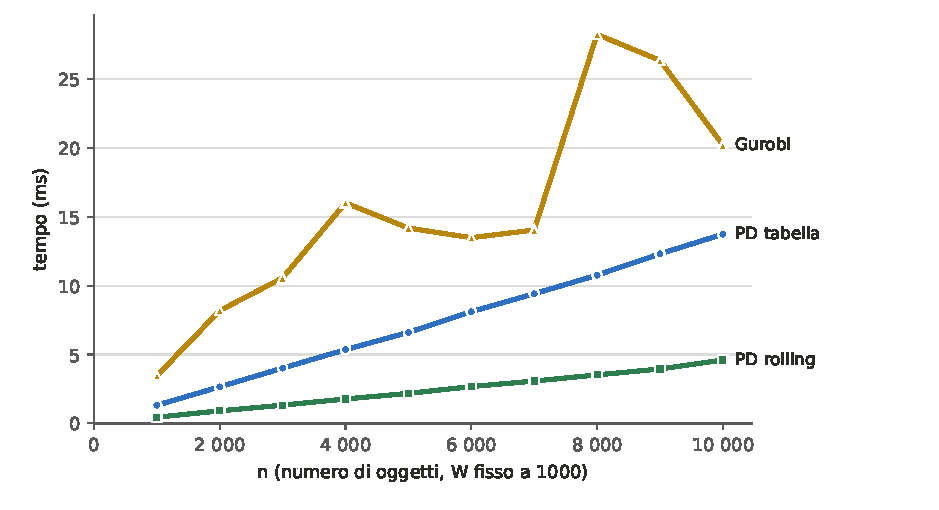
\includegraphics[width=\linewidth]{fig/tempo-vs-n.pdf}
  \caption{Tempo di esecuzione al crescere del numero di oggetti, a capacit\`a
  fissa $W = 1000$.}
  \label{fig:tempo-n}
\end{figure}

\begin{figure}[tbp]
  \centering
  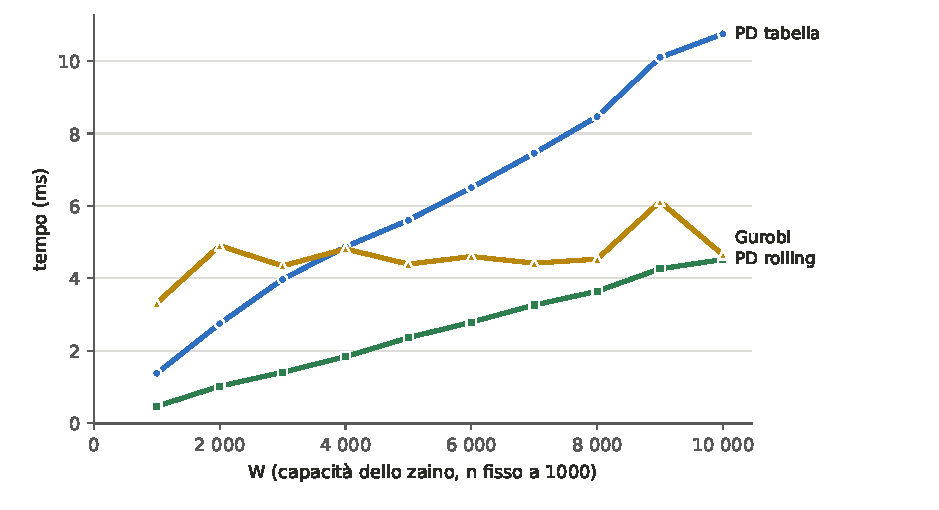
\includegraphics[width=\linewidth]{fig/tempo-vs-W.pdf}
  \caption{Tempo di esecuzione al crescere della capacit\`a, a numero di
  oggetti fisso $n = 1000$.}
  \label{fig:tempo-w}
\end{figure}

Le due campagne coprono lo stesso intervallo di celle calcolate, da un milione a
dieci milioni, ma il costo di una singola cella non \`e il medesimo: circa
$1{,}4$ nanosecondi quando a crescere \`e $n$ e circa $1{,}0$ quando a crescere
\`e $W$, mentre nella variante a spazio ridotto i due valori coincidono; la
differenza \`e imputabile alla struttura della tabella, che in Java \`e un
vettore di riferimenti a righe separate, tante quante gli oggetti.

Quanto alla memoria, nella Figura~\ref{fig:memoria} i valori misurati sull'heap
seguono la formula $(n+1)(W+1)\cdot 8$ byte entro il 5\%, uno scarto attribuibile
alle strutture di servizio della macchina virtuale. La previsione dell'analisi
asintotica \`e quindi confermata anche nella costante, non solo nell'andamento.

\begin{figure}[tbp]
  \centering
  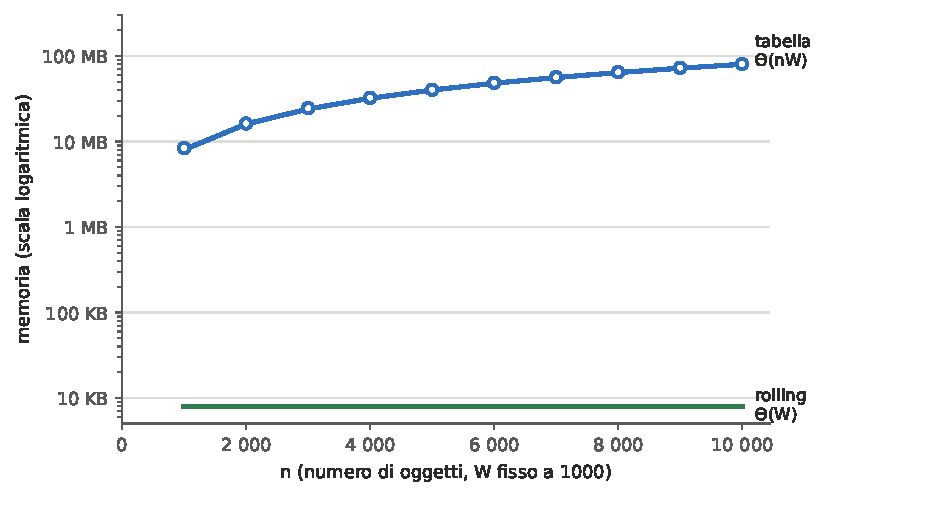
\includegraphics[width=\linewidth]{fig/memoria.pdf}
  \caption{Occupazione di memoria della tabella, calcolata dalla formula (linea)
  e misurata sull'heap (cerchi), a confronto con quella del rolling array. Del
  rolling array \`e riportata la sola formula: la sua occupazione sta sotto la
  soglia di risoluzione della misura.}
  \label{fig:memoria}
\end{figure}

\subsection{Limiti pratici}
La variante a spazio ridotto non serve a essere pi\`u veloce, ma a rendere
trattabili istanze che altrimenti non lo sarebbero. Fissati $n = 2000$ e una
heap di 2~GB, si \`e fatta crescere la sola capacit\`a:

\begin{center}
\begin{tabular}{rrlrl}
\toprule
$W$ & \multicolumn{2}{c}{tabella $\To(nW)$} & \multicolumn{2}{c}{rolling $\To(W)$} \\
\midrule
$100\,000$   & 1,5 GB  & 0,76 s              & 781 KB & 0,09 s \\
$300\,000$   & 4,5 GB  & memoria esaurita    & 2,3 MB & 0,27 s \\
$1\,000\,000$ & 14,9 GB & memoria esaurita   & 7,6 MB & 0,92 s \\
\bottomrule
\end{tabular}
\end{center}

\noindent
Gi\`a a $W = 300\,000$ l'algoritmo base non arriva in fondo, mentre la variante
risolve la stessa istanza usando due megabyte e un quarto di secondo. \`E il
risultato richiesto dal Compito~2: a parit\`a di tempo asintotico, la riduzione
dello spazio estende di oltre un ordine di grandezza le capacit\`a trattabili.

\subsection{Confronto con il solver}
Su tutte le istanze provate il valore ottimo calcolato dalla programmazione
dinamica coincide con quello del solver: il riscontro esterno di correttezza \`e
soddisfatto. Sui tempi i due si comportano diversamente e nessuno dei due domina
l'altro. Al crescere del numero di oggetti la programmazione dinamica \`e pi\`u
veloce e, soprattutto, prevedibile: il suo tempo \`e determinato da $n$ e $W$,
mentre quello del solver dipende da quanto l'istanza si presta ai tagli e alle
riduzioni del branch and bound, e nelle misure oscilla in modo non monotono. Al
crescere della capacit\`a le parti si invertono: per il solver $W$ \`e soltanto
un coefficiente del vincolo, mentre per la programmazione dinamica \`e una
dimensione della tabella.

\subsection{Riproduzione degli esperimenti}
Il codice si compila con lo script fornito e non richiede altro che una macchina
virtuale Java; il modulo del solver viene incluso soltanto se la libreria \`e
raggiungibile. I comandi principali sono i seguenti.

\begin{codice}
\begin{Verbatim}[fontsize=\small]
./compile.sh                      compila in bin/
java -cp bin knapsack.Main test   batteria di correttezza

java -cp bin knapsack.Main generate 200 5000 42 -o istanza.txt
java -cp bin knapsack.Main solve istanza.txt --dump-table tabella.csv
java -cp bin knapsack.Main solve istanza.txt --rolling

java -Xms2g -Xmx2g -cp bin knapsack.Main bench nsweep \
     --fixed 1000 --from 1000 --to 10000 --step 1000 --reps 7 -o dp_n.csv

./campagna.py                     rifa l'intera campagna in data/campagna/
./grafici.py                      rifa le figure di questa relazione
\end{Verbatim}
\end{codice}

\noindent
L'opzione \texttt{-{}-dump-table} salva la tabella $K$ in formato CSV, cos\`i che
il contenuto prodotto dal primo algoritmo sia disponibile per un'ispezione
diretta. I file CSV della campagna fanno parte del materiale consegnato e si
aprono con un foglio di calcolo.

% ============================================================
\section{Limitazioni e conclusioni}

\subsection{Limitazioni riscontrate}
La misura della memoria sull'heap ha una risoluzione dell'ordine del mezzo
megabyte, imposta dalla granularit\`a con cui la macchina virtuale alloca:
sufficiente per la tabella, che ne occupa decine, inutilizzabile per la variante
a spazio ridotto, i cui pochi kilobyte restano sotto la soglia. Di quest'ultima
si riporta perci\`o la sola occupazione calcolata, che \`e comunque esatta.

La variante a spazio ridotto perde la ricostruzione della soluzione e ne
restituisce il solo valore. Esiste una tecnica, dovuta a Hirschberg, che
recupera la soluzione mantenendo lo spazio $\To(W)$ a prezzo di un fattore
costante sul tempo, dividendo ricorsivamente il problema attorno a un punto di
taglio; non \`e stata implementata, e resta lo sviluppo naturale del lavoro.

Le misure provengono da una sola macchina e da una sola macchina virtuale: gli
andamenti sono affidabili, i valori assoluti no. Le istanze sono generate con
pesi e valori indipendenti e uniformi, che non coprono le famiglie note per
essere difficili per i metodi di enumerazione implicita, come quelle in cui il
valore \`e proporzionale al peso; il confronto con il solver va quindi letto per
quello che \`e, un termine di paragone esterno su istanze casuali, e non come
uno studio sistematico del solver.

\subsection{Conclusioni}
I tre compiti sono stati svolti sul problema dello Zaino 0/1: la programmazione
dinamica \`e applicabile perch\'e valgono entrambi i criteri, sottostruttura
ottima e sovrapposizione dei sottoproblemi; i due algoritmi sono stati scritti,
analizzati e codificati; la sperimentazione ne ha confrontato la crescita
empirica con l'analisi asintotica.

Il risultato che vale la pena trattenere \`e duplice. Da un lato l'analisi
prevede il comportamento osservato con precisione insolita: il tempo cresce
linearmente in ciascuno dei due fattori e la memoria segue la formula entro il
5\%, senza sorprese legate ai dati, perch\'e l'algoritmo percorre comunque tutte
le celle. Dall'altro il fattore che decide quali istanze siano davvero
trattabili non \`e il numero di oggetti ma la capacit\`a, ed \`e sulla memoria,
non sul tempo, che il limite si presenta per primo: da qui l'utilit\`a concreta
della variante a spazio ridotto, che sposta quel limite di oltre un ordine di
grandezza.

\end{document}
